\documentclass[preprint,12pt,authoryear,review]{elsarticle}

\usepackage{amssymb}

% custom
\usepackage{amsmath}
\newcommand*{\norm}[1]{\left\lVert#1\right\rVert}
\newcommand{\argmin}{\arg\!\min}

\usepackage[bottom]{footmisc}
\usepackage[dvipsnames]{xcolor}
\usepackage[colorlinks]{hyperref}
\hypersetup{citecolor=blue, citebordercolor={1 1 1}}
\usepackage[capitalise]{cleveref}
\usepackage{mathtools}
\usepackage{nth}
\usepackage{siunitx}

\usepackage{lineno}

\usepackage{soul}

\renewcommand{\figurename}{SI Figure}
\renewcommand{\thefigure}{S\arabic{figure}}


\begin{document}

	\noindent \textbf{Supplementary Information for}

	\begin{center}
		Accelerated Diffusion Magnetic Resonance Imaging at 7~T: \\
		Joint Reconstruction
		for Multi-Band Multi-Shell Shift-Encoded \\
		Echo Planar Imaging (JETS-EPI)
	\end{center}

	\begin{center}
		Z. Tan, P. A. Liebig, R. M. Heidemann, F. B. Laun, F. Knoll
	\end{center}

	\vspace{3em}

	\tableofcontents

	\clearpage

	% ============================================ %
	\section{Investigating Iteration Steps and $\rho$ in ADMM}

	We used the data acquired with single-shell encoding and \SI{1.2}{\milli\meter} isotropic resolution to demonstrate the effects of ADMM iteration steps and the coupling scalar $\rho$
	on convergence.


	\begin{figure}[h!]
		\centering
		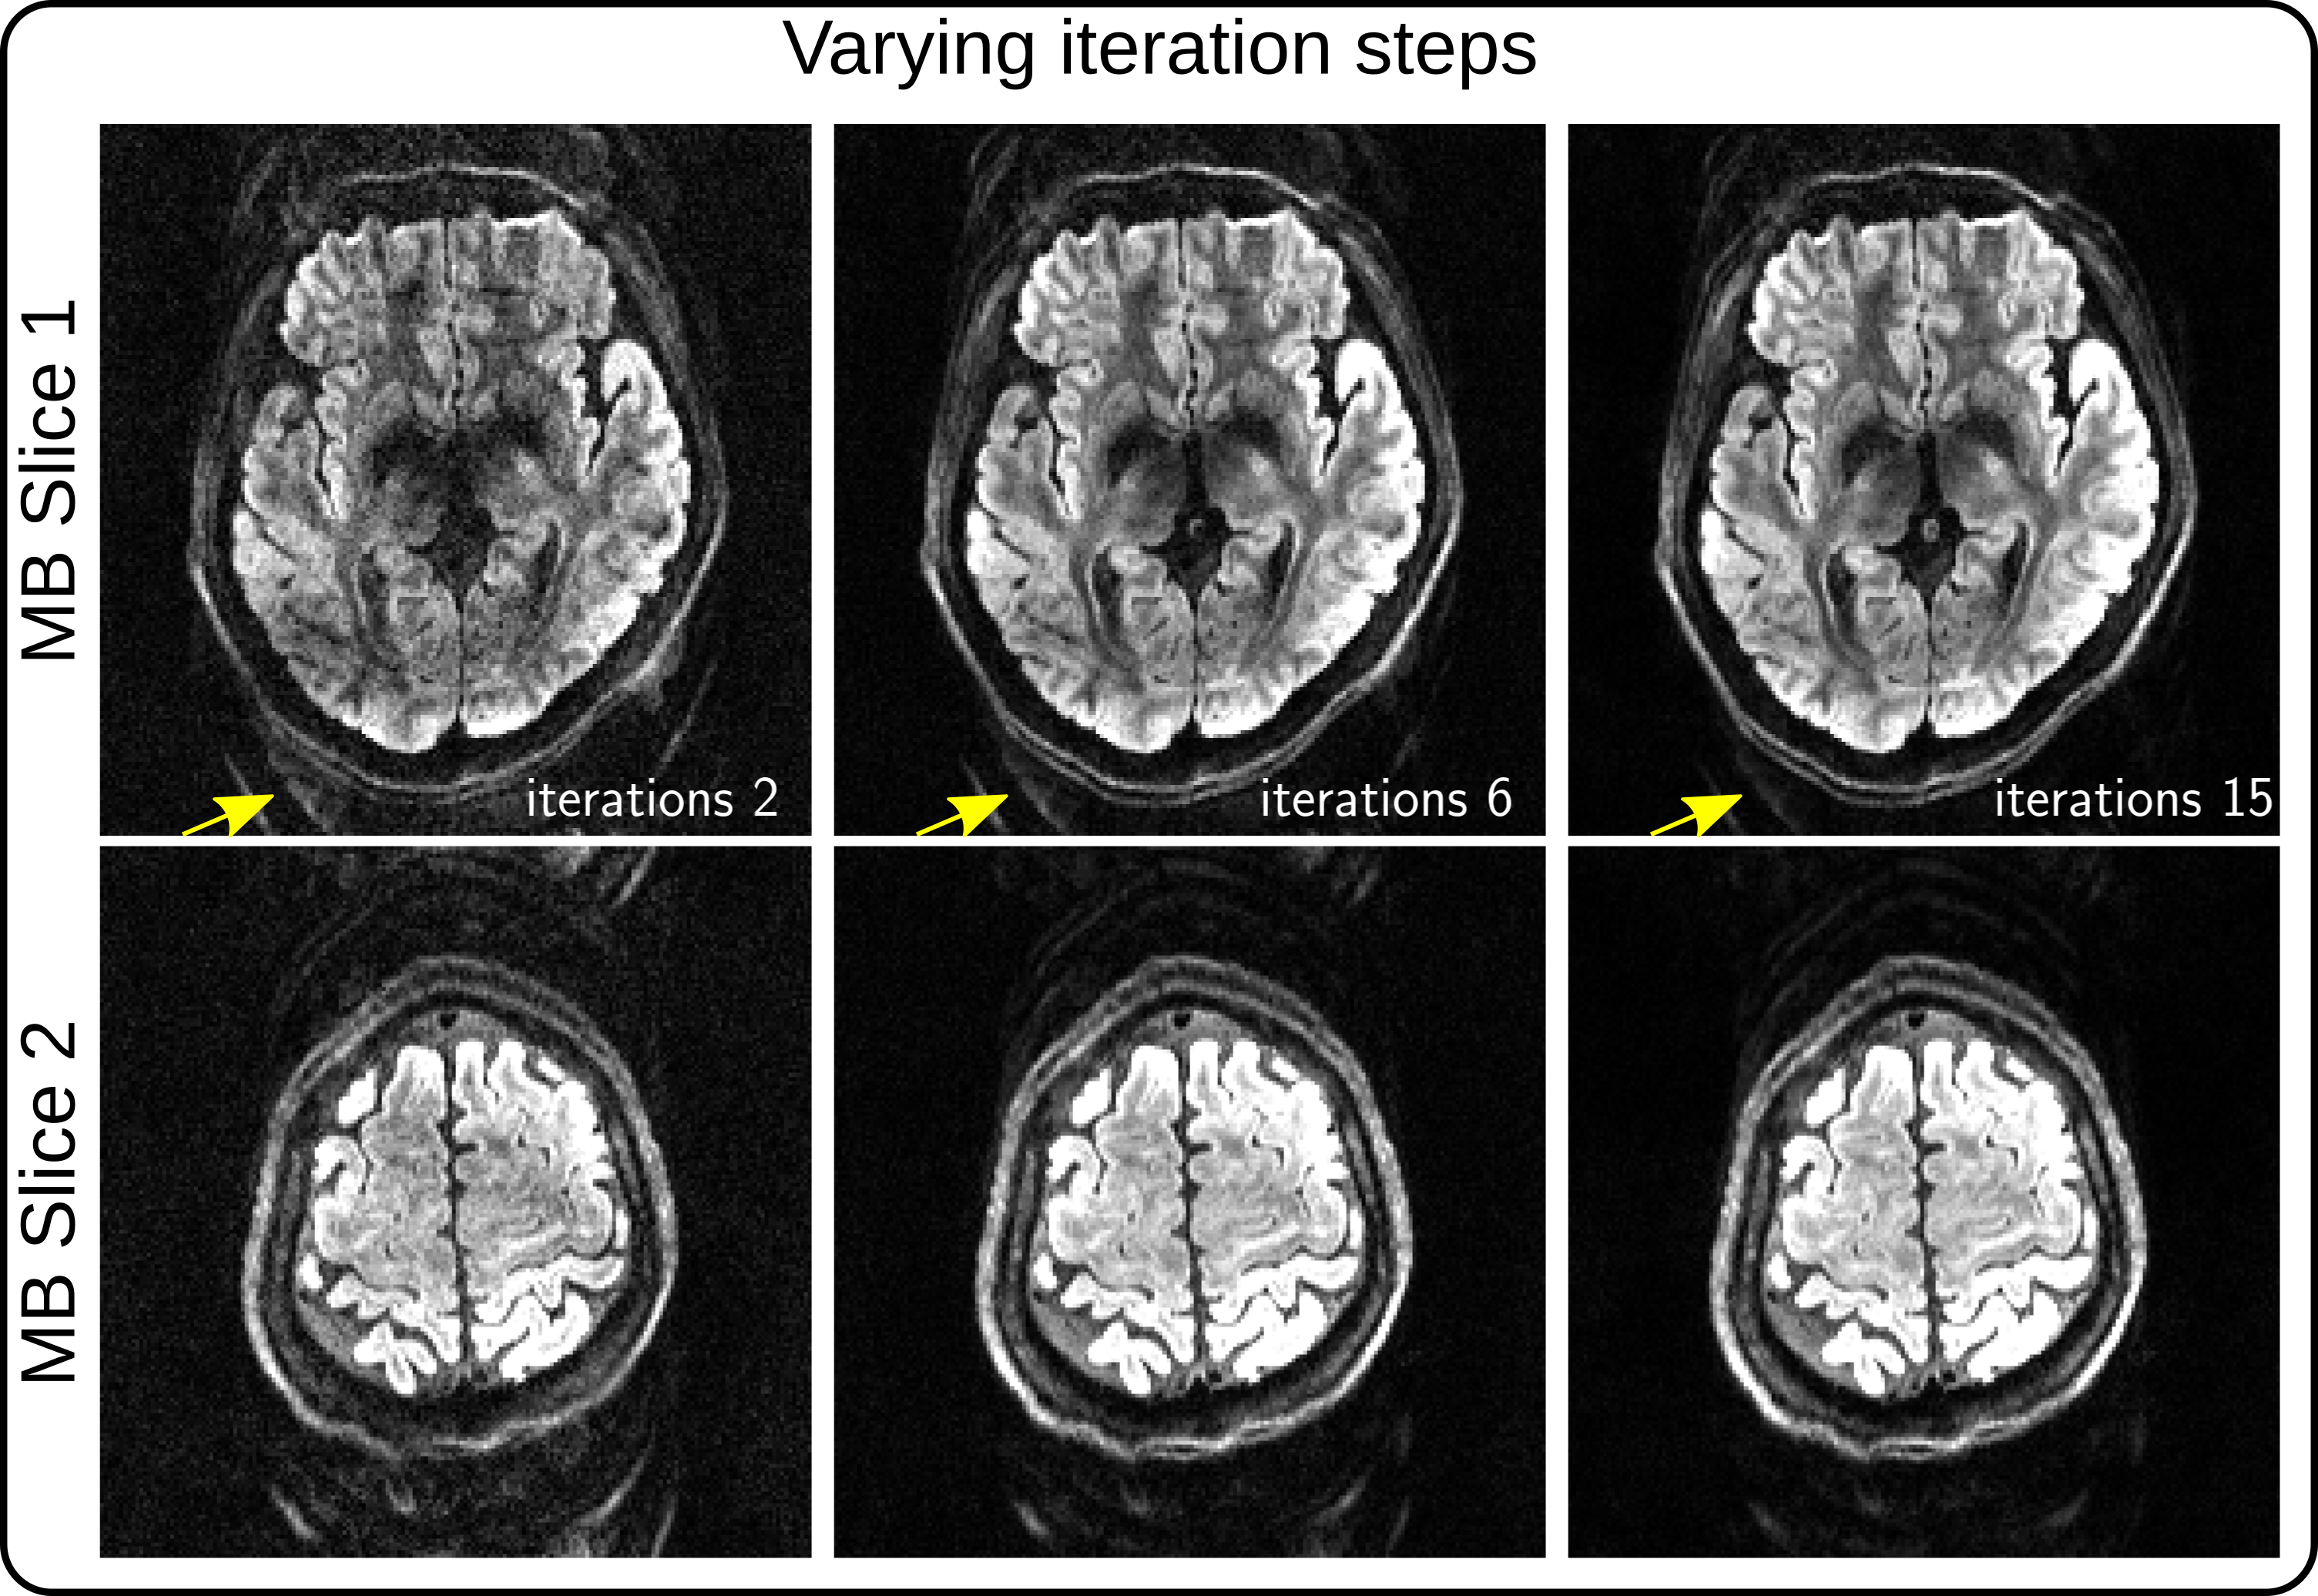
\includegraphics[width=\textwidth]{../figures/supp_fig1.png}
		\caption{Investigation of ADMM convergence with varying iteration steps
			while keeping $\rho = 0.05$ and $\lambda = 0.04$.
			Reconstructed multi-band diffusion-weighted images at the \nth{11} diffusion encoding
			with 2, 6, and 15 ADMM iterations are displayed from left to right, respectively.
			Inadequate iteration suffers from residual aliasing artifacts due to undersampling
			(indicated by yellow arrows).}
		\label{FIG:conv_iter}
	\end{figure}

	\begin{figure}[h!]
		\centering
		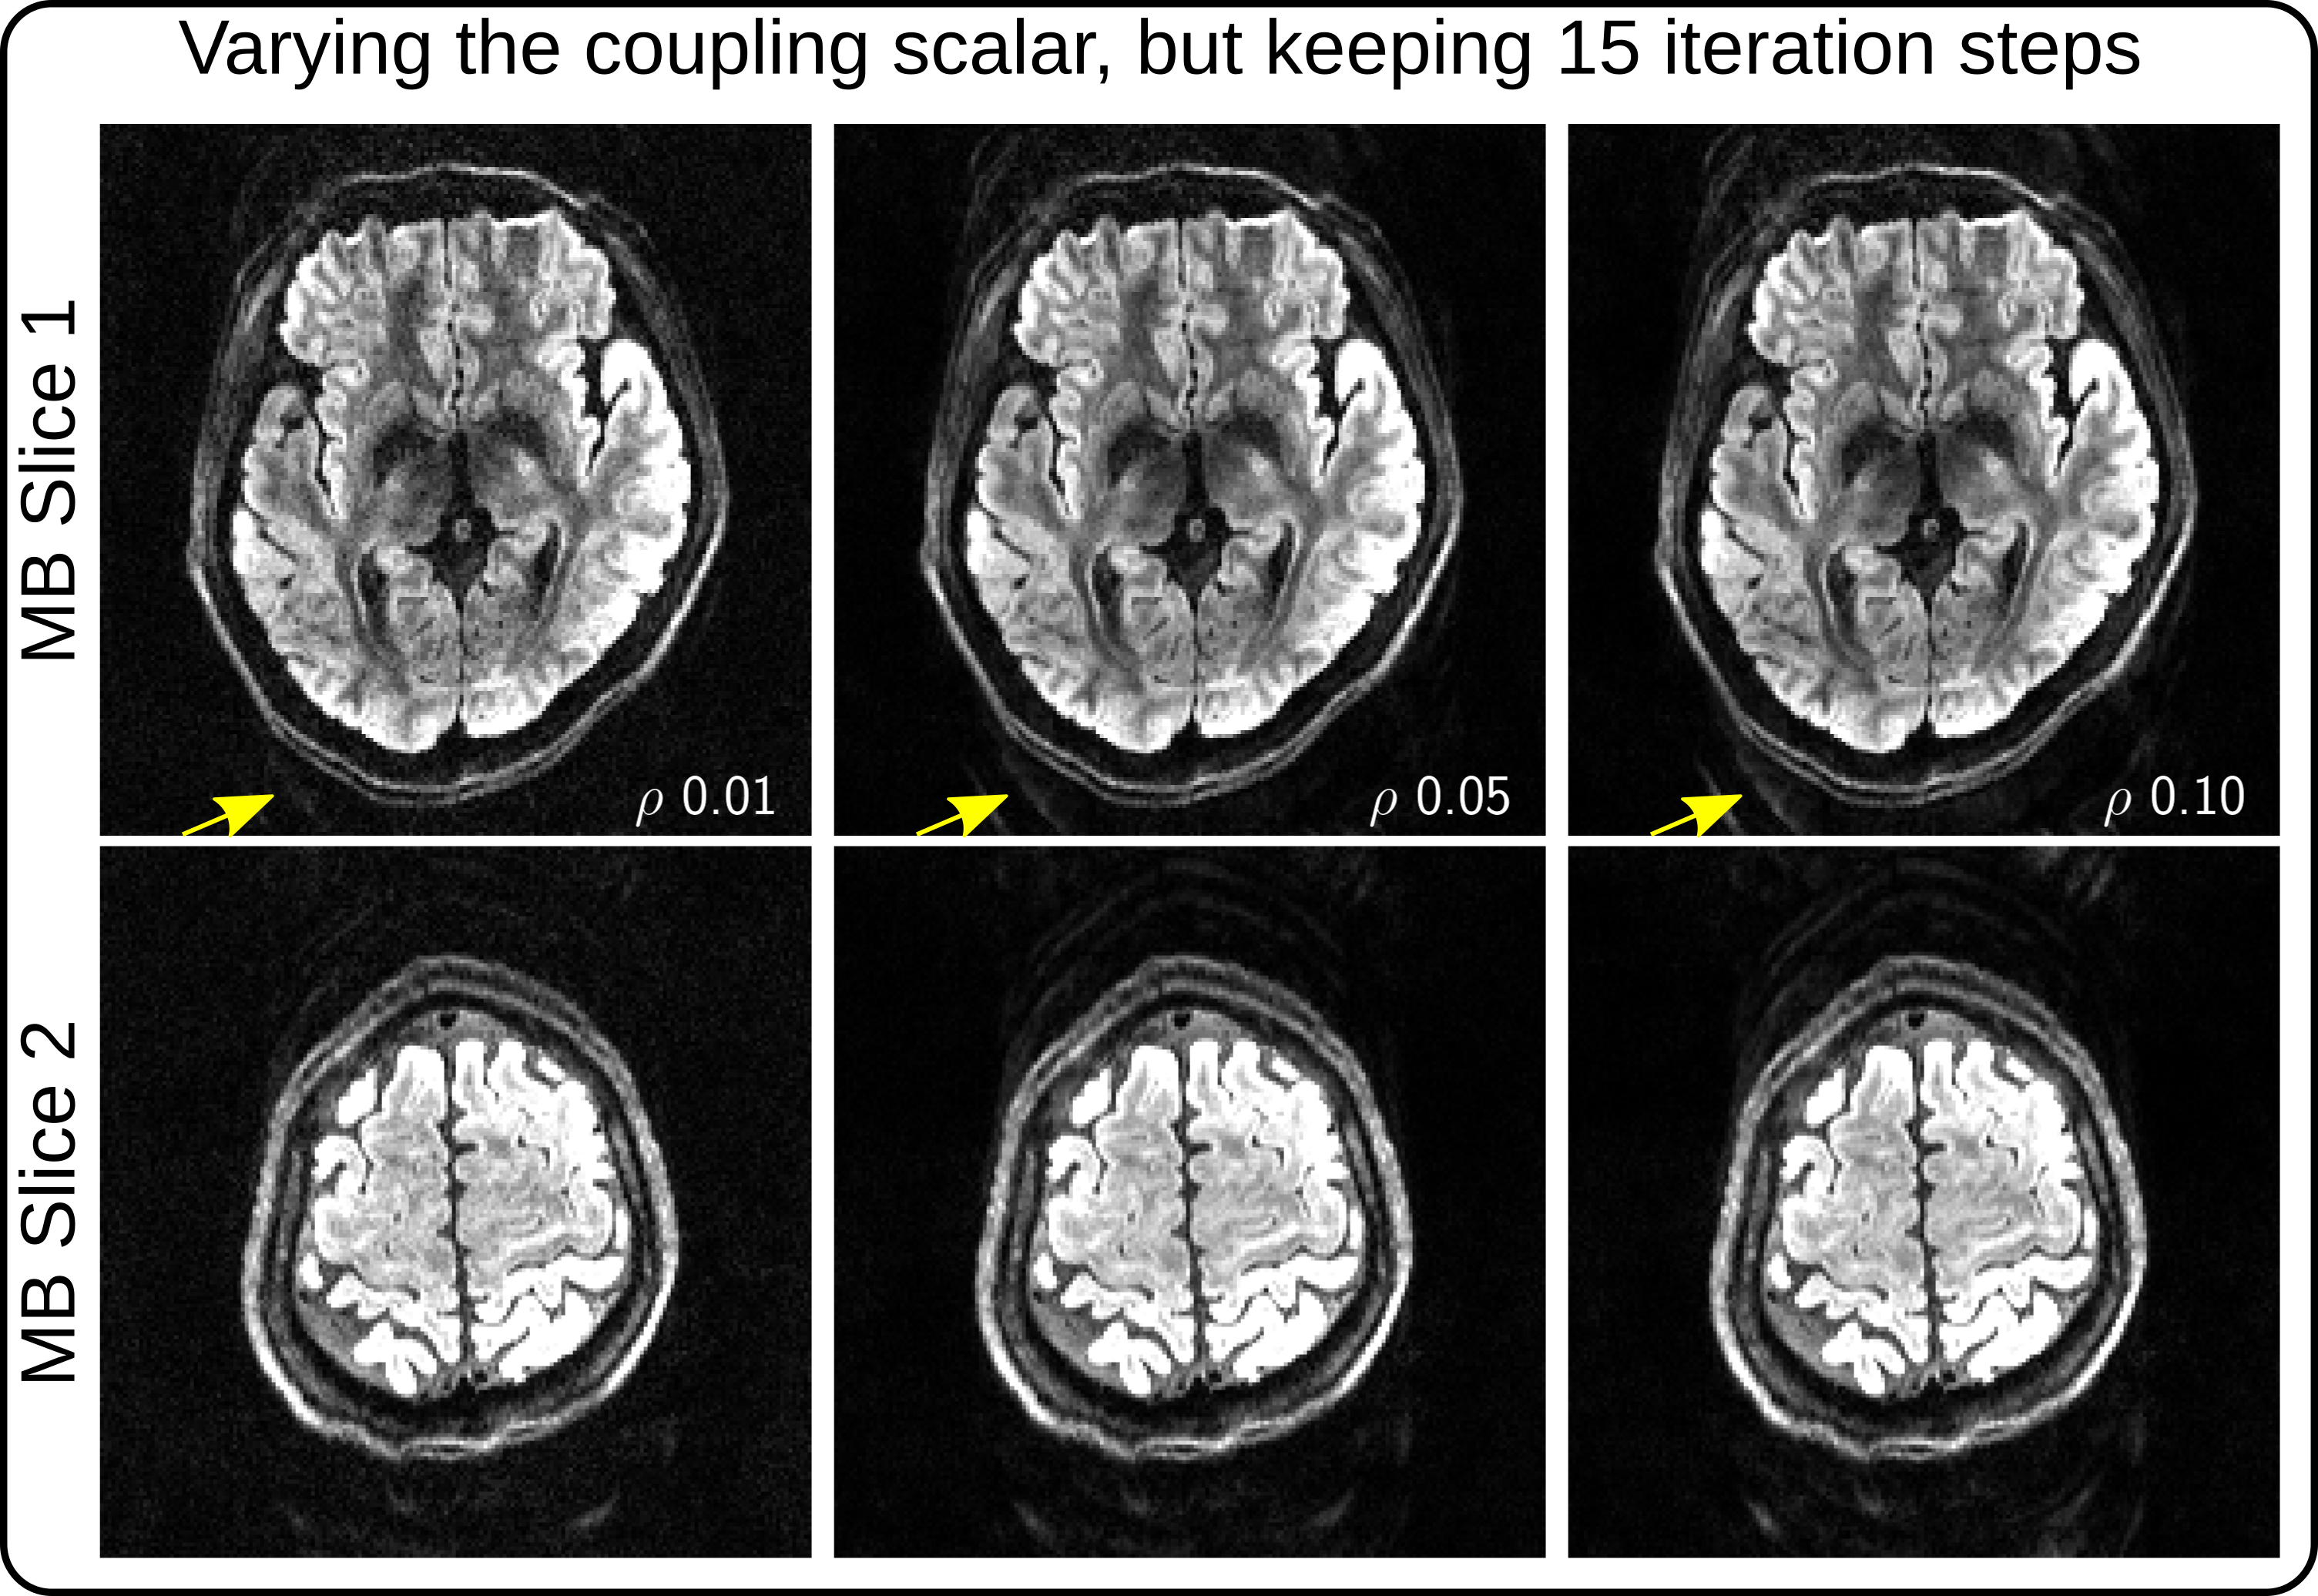
\includegraphics[width=\textwidth]{../figures/supp_fig2.png}
		\caption{Investigation of ADMM convergence with varying $\rho$
			while keeping 15 iteration steps and $\lambda = 0.04$.
			Reconstructed multi-band diffusion-weighted images at the \nth{11} diffusion encoding
			with $\rho$ as $0.01$, $0.05$, and $0.10$ are displayed from left to right, respectively.
			As indicated by yellow arrows, smaller $\rho$ ($0.01$) supplies less aliasing artifacts
			compared to larger $\rho$ ($0.10$), but also shows more noise.}
		\label{FIG:conv_rho}
	\end{figure}

	\clearpage

	% ============================================ %
	\section{Investigating Block Size in LLR Regularization}

	\begin{figure}[h!]
		\centering
		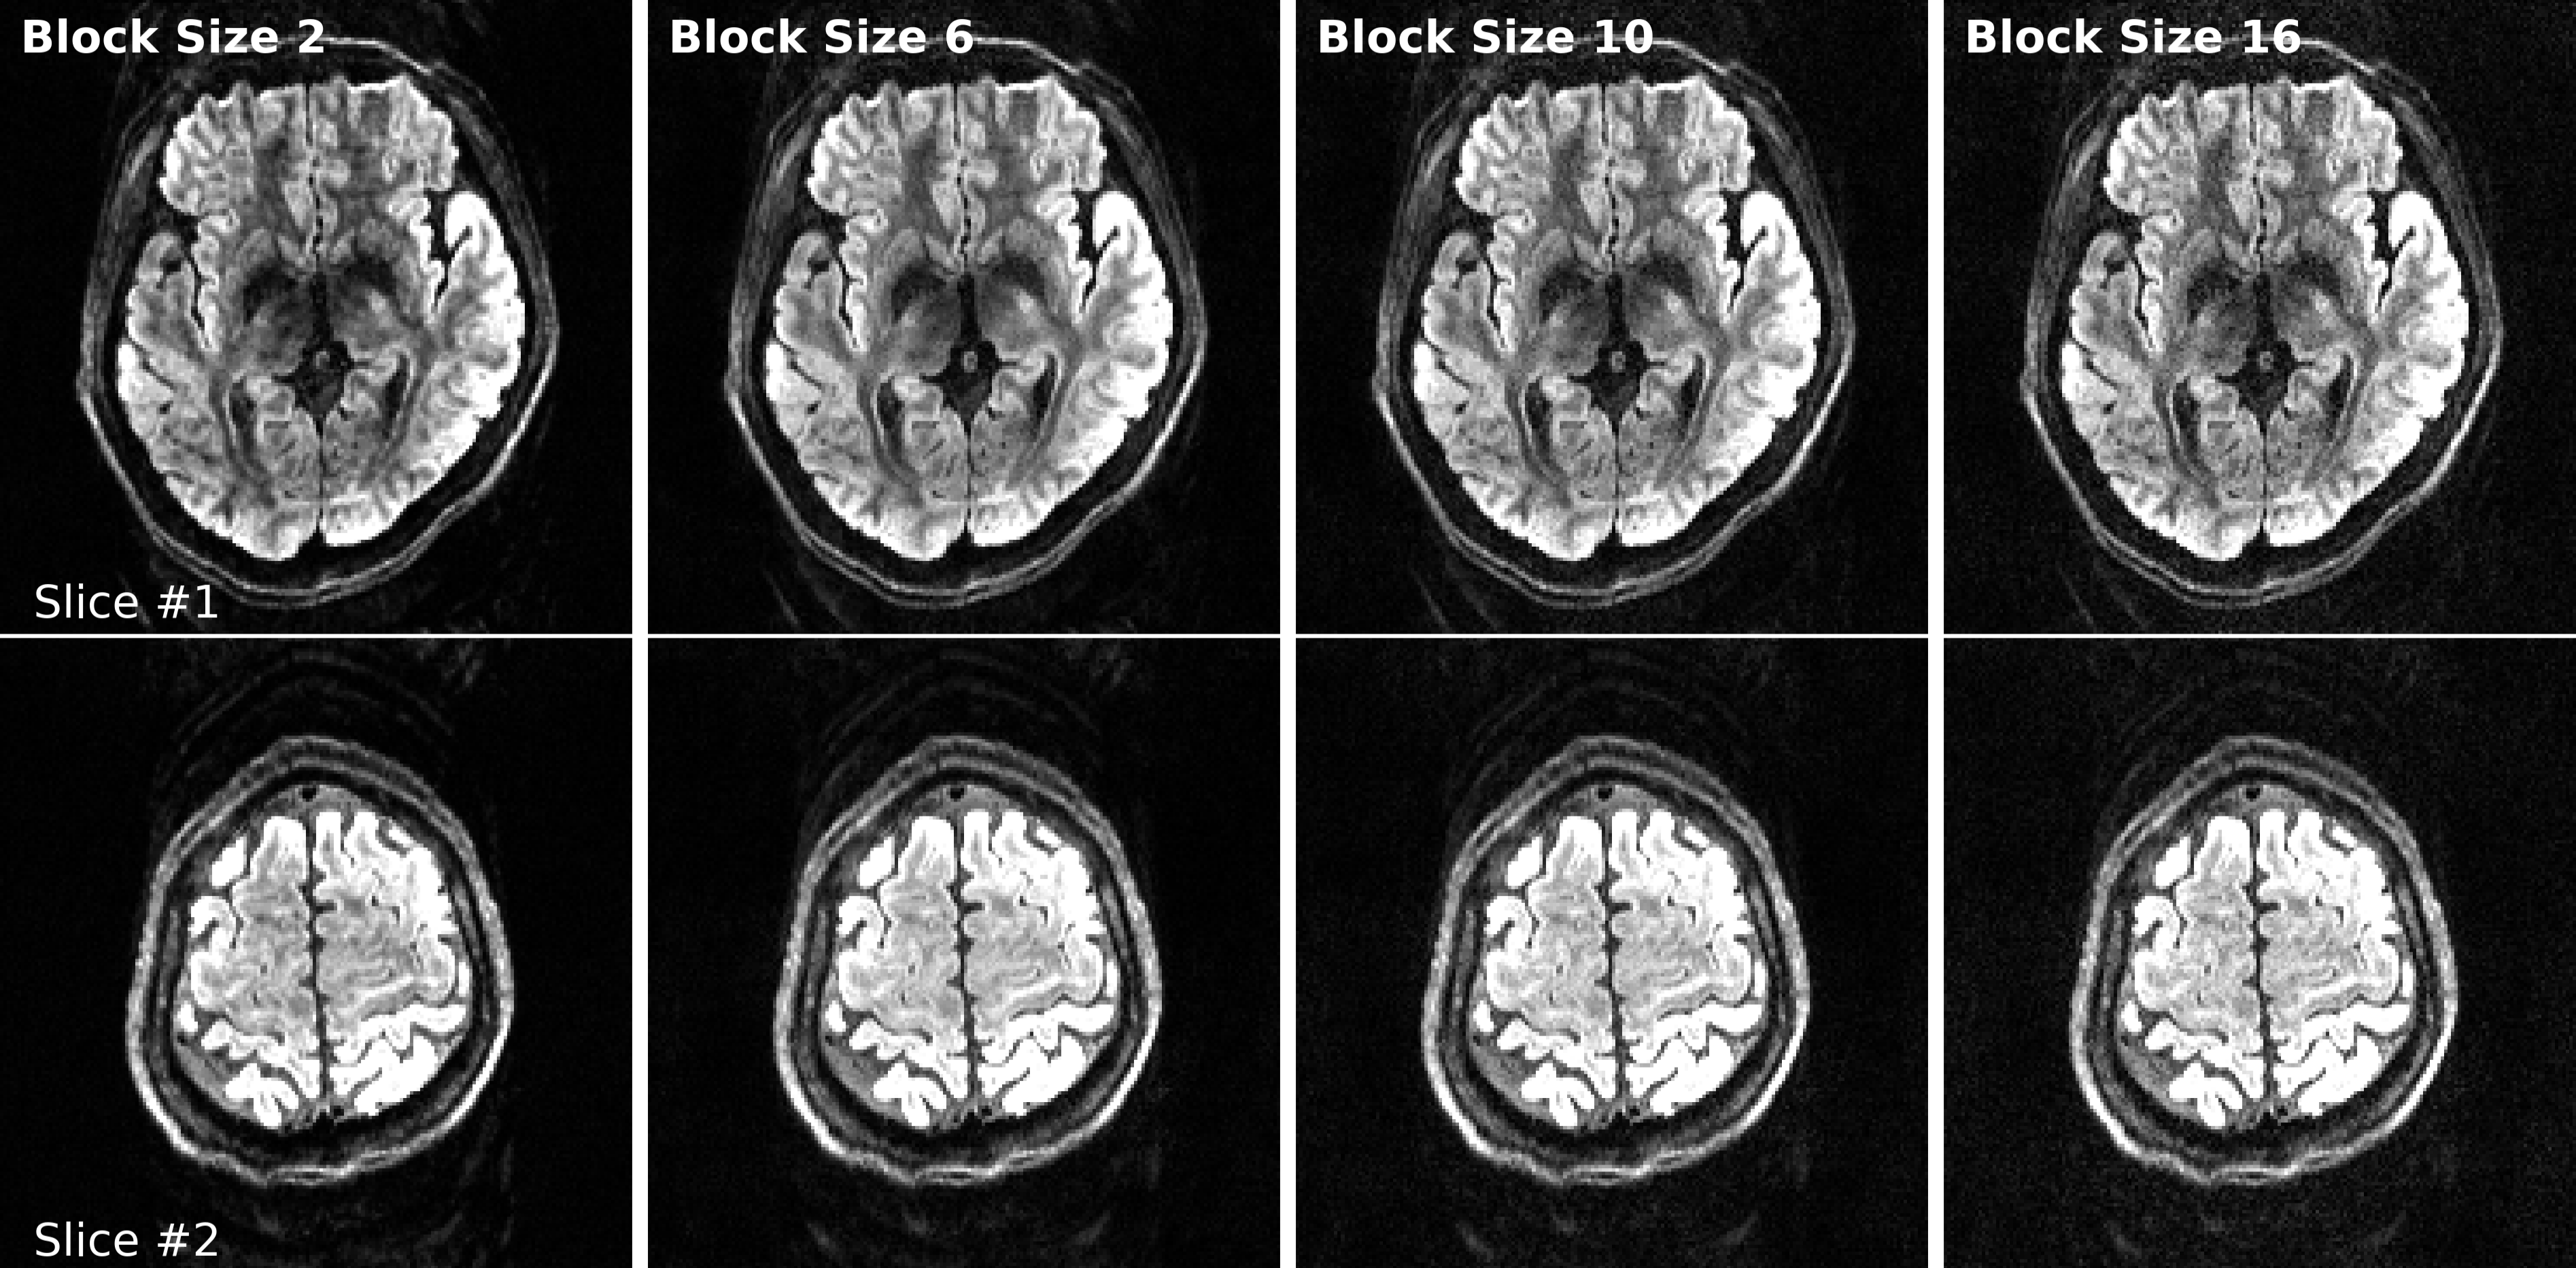
\includegraphics[width=\textwidth]{../figures/supp_fig3.png}
		\caption{Investigation of block size in LLR regularization.
			Reconstructed multi-band diffusion-weighted images
			at the \nth{11} diffusion encoding with block sizes as 2, 6, 10, and 16
			from left to right, respectively.
			Small block size (i.e., 2) suffers from image blurring,
			whereas increasing block size gradually leads to increased noise.
			Therefore, block size of 6 is used in this work.}
		\label{FIG:blocks}
	\end{figure}

	\clearpage


	% ============================================ %
	\section{Reproducing MUSE and MUSSELS in Python}

	For the use of the state-of-the-art multi-echo EPI diffusion MRI reconstruction techniques,
	i.e.~MUSE and MUSSELS, we firstly reproduce these techniques in Python based on open source codes and data.

	\vspace{2em}

	\begin{figure}[h]
		\centering
		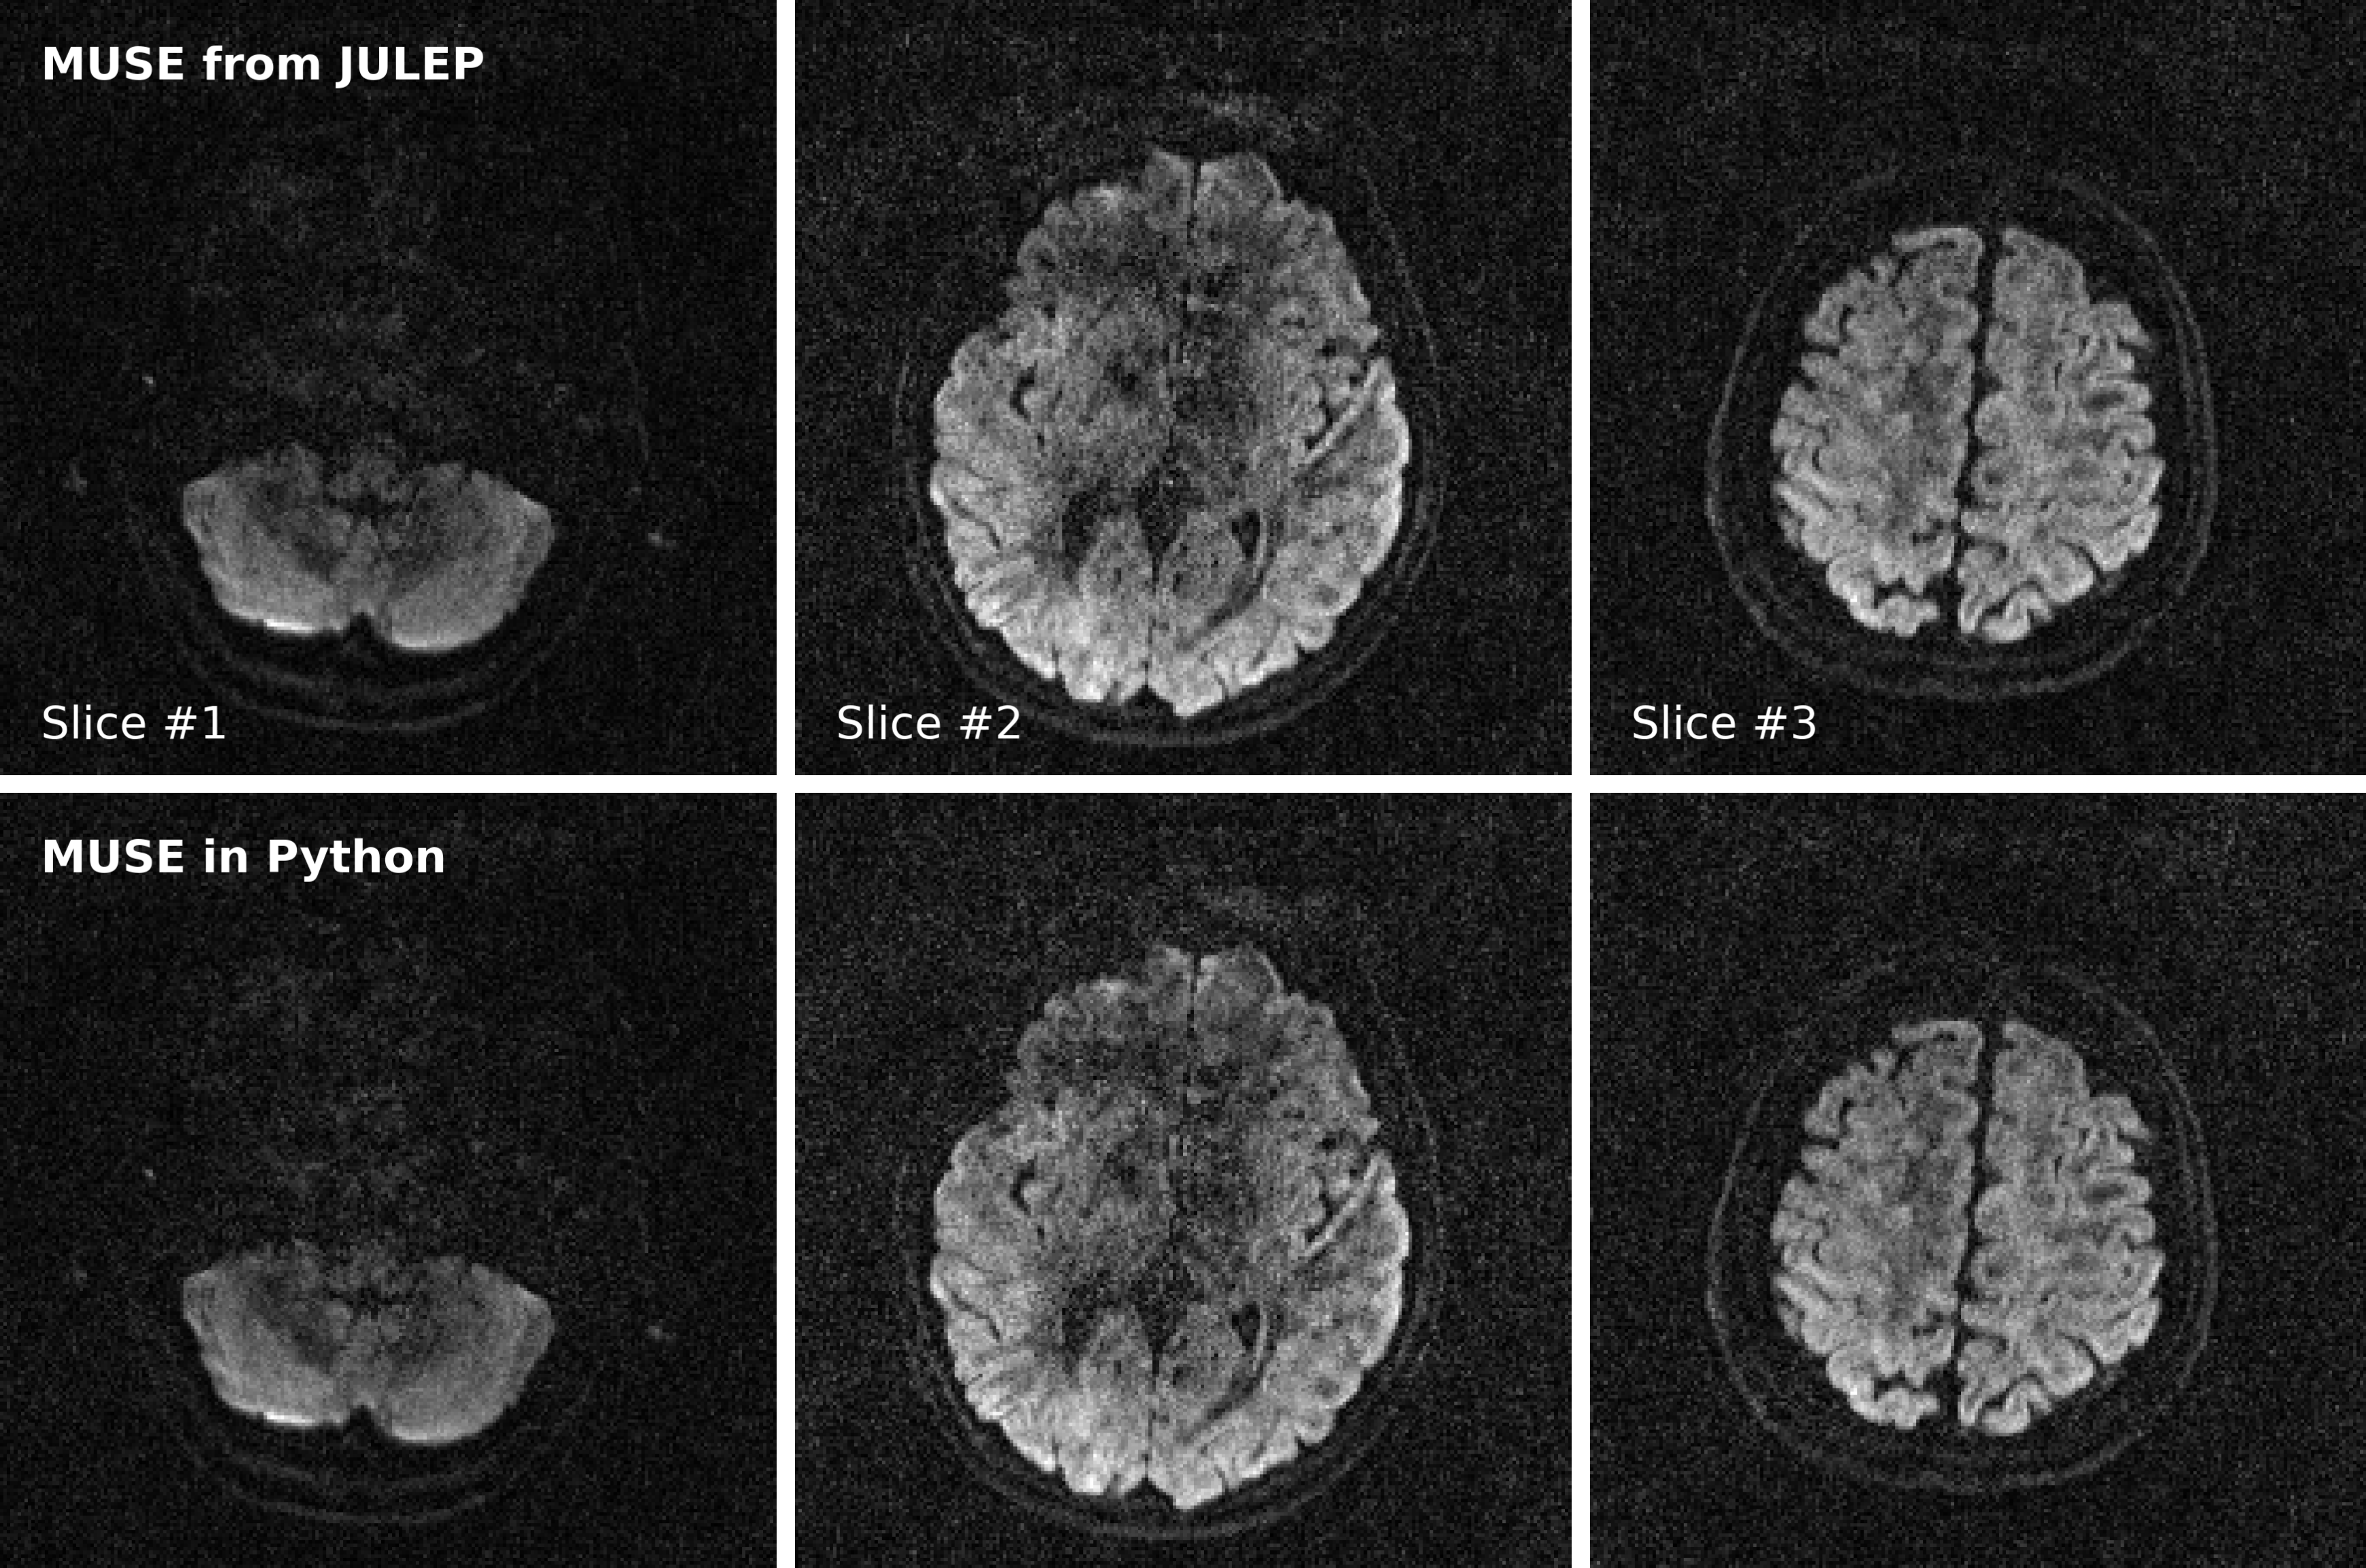
\includegraphics[width=\textwidth]{../figures/supp_fig4.png}
		\caption{Reproduce MUSE from the source code and data from JULEP
			(\url{https://github.com/daiep/JULEP}).
			This data is acquired by 4-shot interleaved EPI with
			in-plane acceleration factor per shot being 4 and
			multi-band factor being 3.
			The top and bottom rows display the reconstruction results of MUSE from JULEP
			and our Python implementation, respectively.
			With this comparison, we validate our Python implementation,
			which is then served for the MUSE reconstruction of our \SI{7}{T} data
			in this work.
		}
		\label{FIG:reprod_muse}
	\end{figure}

	\begin{figure}[h!]
		\centering
		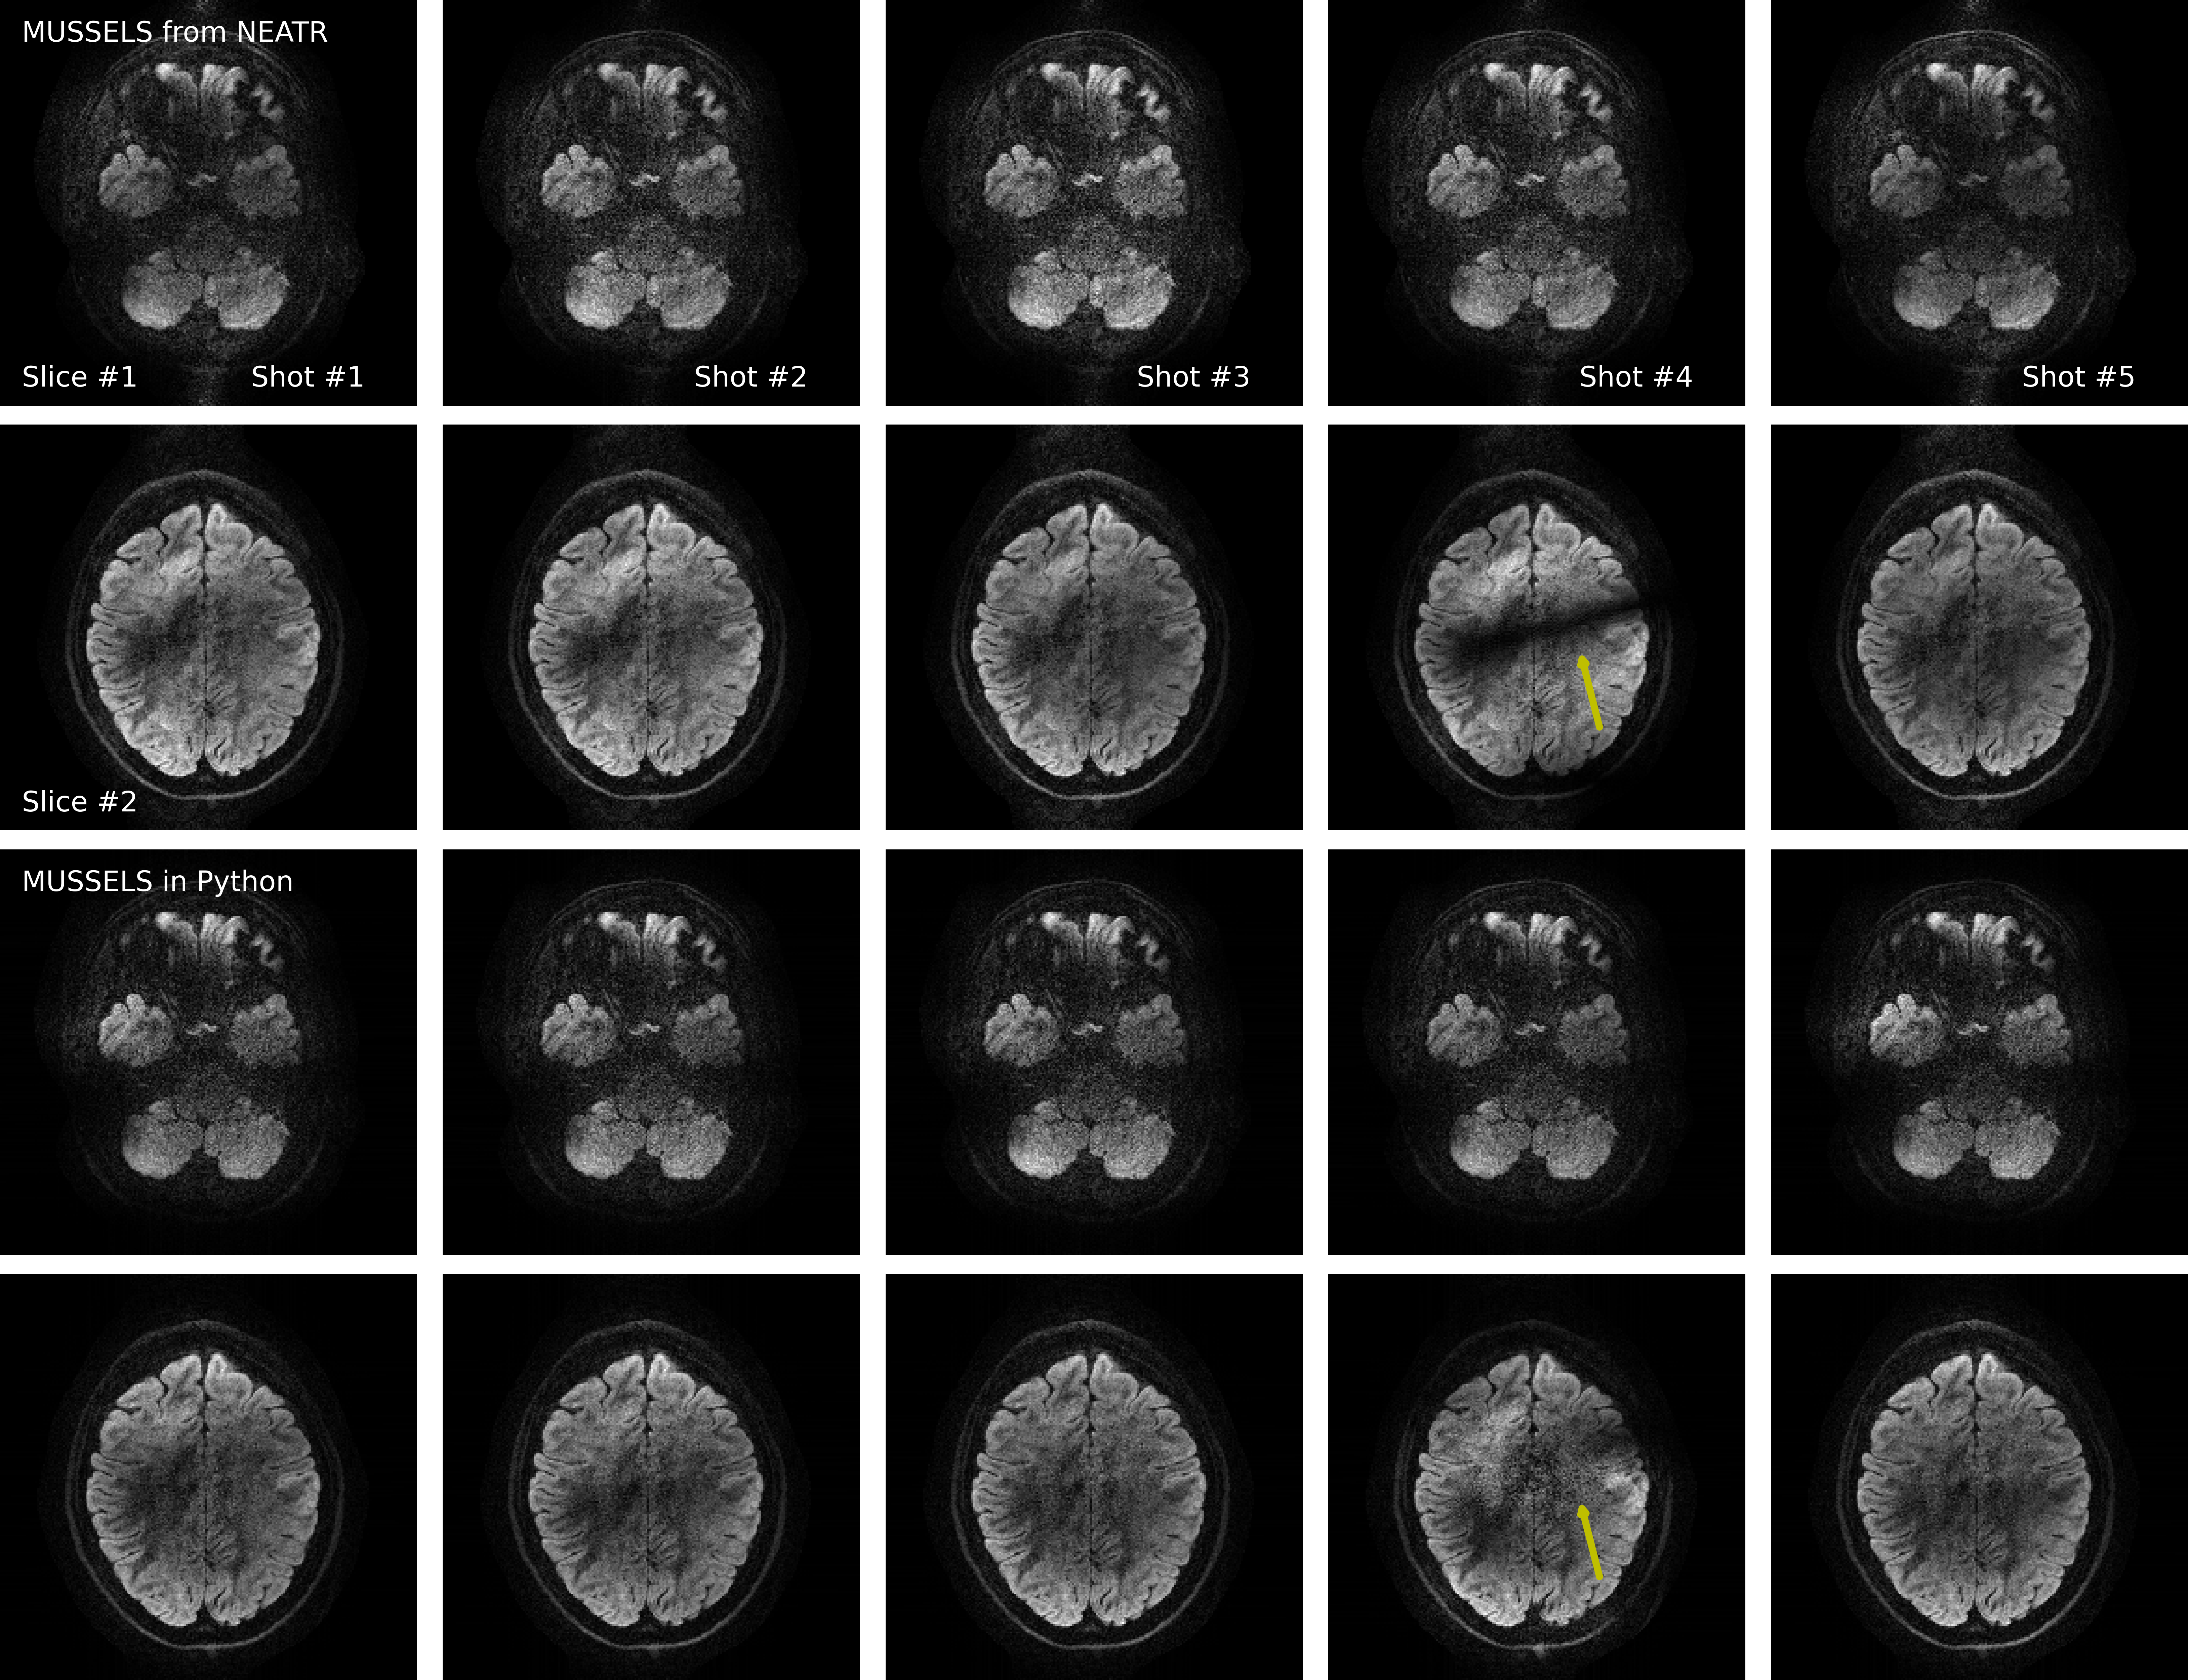
\includegraphics[width=\textwidth]{../figures/supp_fig5.png}
		\caption{Reproduce MUSSELS based on the data from NEATR
			(\url{https://bit.ly/2QgBg9U}).
			The data is acquired by 9-shot interleaved EPI with multi-band factor being 2.
			5 shots are extracted from this data for MUSSELS reconstruction.
			Therefore, the in-plane acceleration factor per shot is 9.
			The top two rows present the MUSSELS reconstruction results based on the implementation in NEATR, whereas the bottom two rows present our Python implementation.
			Note that the MUSSELS implementation from NEATR shows artifacts in the 4th shot image of the second slice. }
		\label{FIG:reprod_mussels}
	\end{figure}

	\clearpage

	% ============================================ %
	\section{Supporting Results from Diffusion Acquisition with Three-Shell Encoding and 1~mm Isotropic Resolution}

	\begin{figure}[h!]
		\centering
		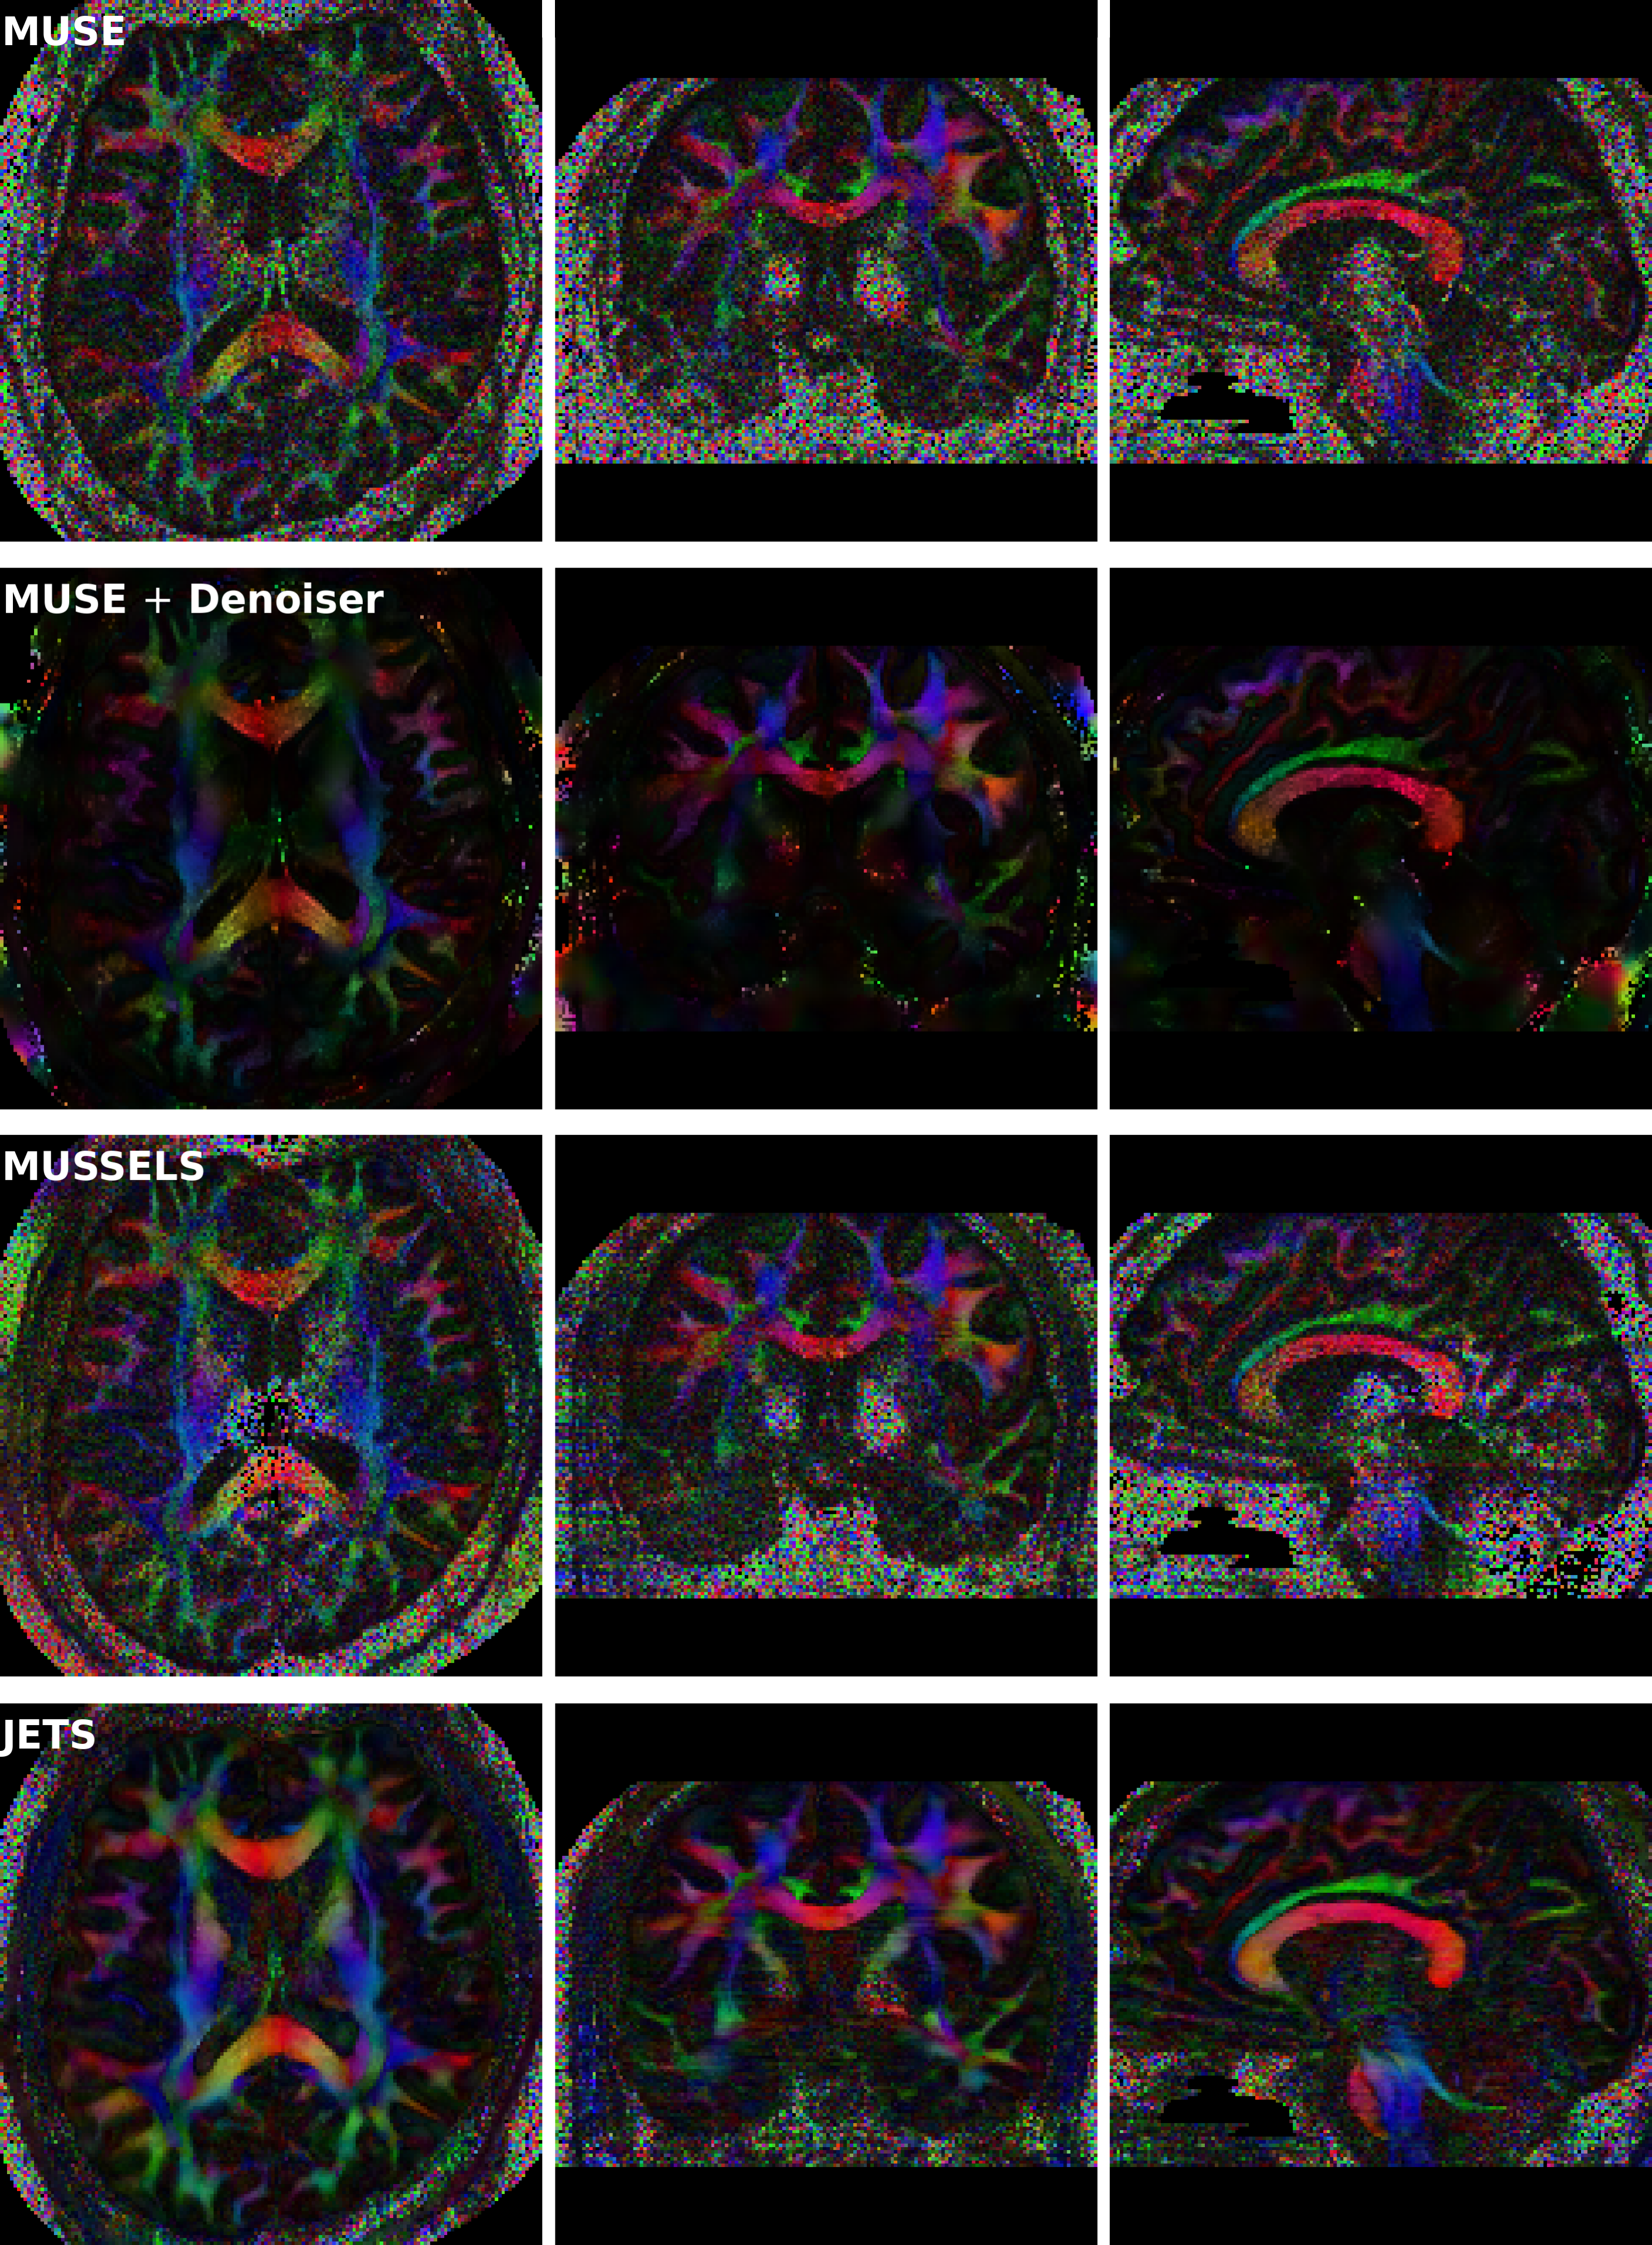
\includegraphics[width=0.85\textwidth]{../figures/supp_fig6.png}
		\caption{Comparison of reconstructed color-coded FA maps
		based on \SI{1}{mm}.}
		\label{FIG:1.0mm_cFA}
	\end{figure}

\end{document}
